\documentclass{article}
\usepackage{stackengine}
\usepackage{graphicx}
\usepackage{caption}
\def\delequal{\mathrel{\ensurestackMath{\stackon[1pt]{=}{\scriptstyle\Delta}}}}
\raggedright

\begin{document}
\today
\tableofcontents


\section{Data description and Visualisation}\label{sec: Descript_visual} % (fold)


\begin{figure}[htbp]
    \centering
    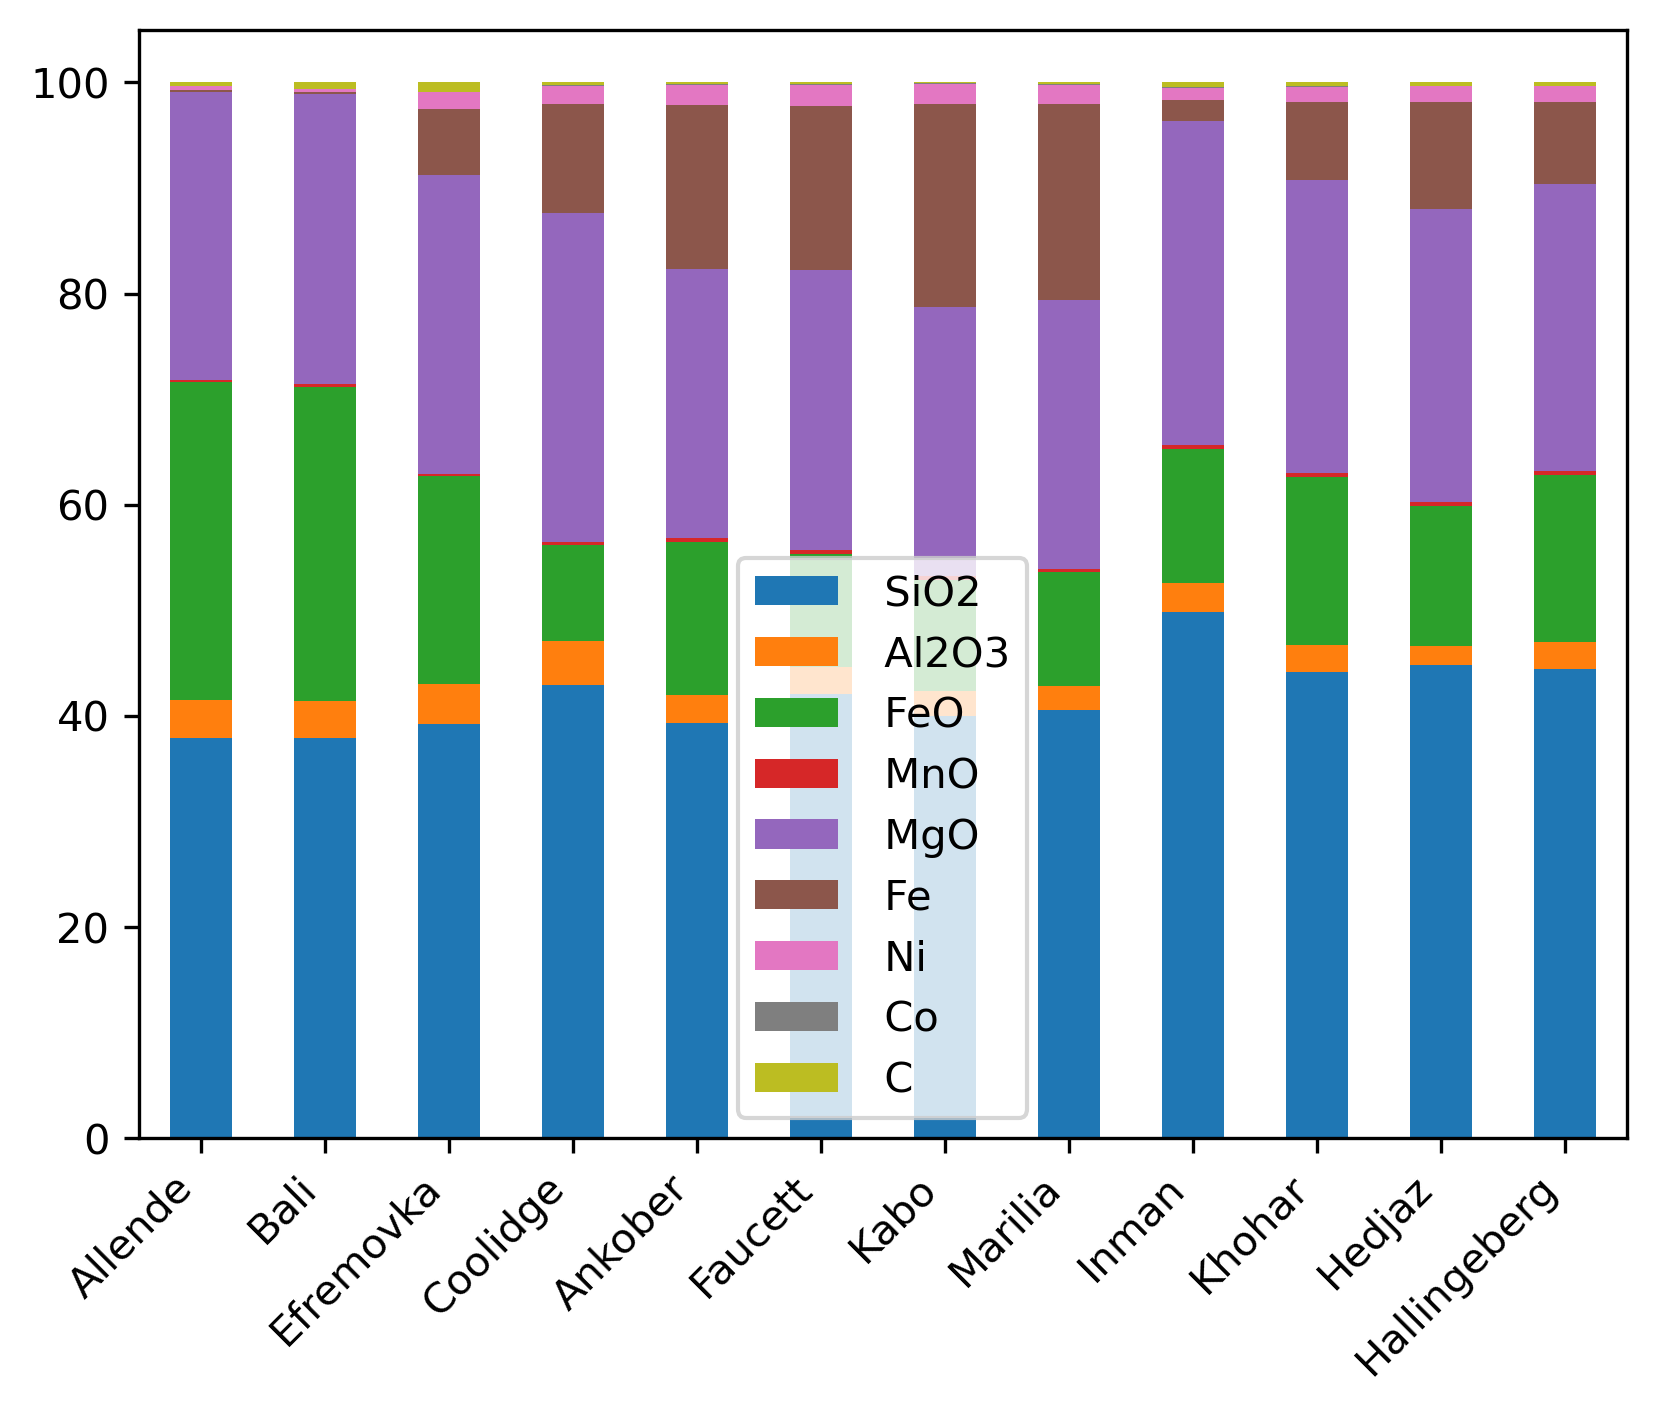
\includegraphics[width=0.8\textwidth]{figures/stacked_bar.png}
    \caption{Example plot showing the chemical composition of meteorites.}
    \label{fig:stacked}
\end{figure}



% section  (end)


\newpage{}

\section{Notes}

Deadline: 12/5 kl. 14

5-10 pages incl. Figures

No collaboration

Dataset 1: Simple. No zeros. Maybe look up usage of antibitoics in each country.

Dataset 2: Simple. No zeros. Look up metadata: cc, hc, lc \newline

Dataset 3: Medium. Last column: metadata. Lots of zeros. Maybe mislabelling because of mistakes from people handling the data.\newline

\textbf{Diet of African Hominidae}
Fecal metagenomes from Chimps and human children from Africa. Samples have been mapped against a mitochondrial database and a subset of genera is given as parts. 2 genera refer to the host and the rest are assumed to refer to the diet. Lots of zeros and possibly mismappings and mislabelled samples. Complexity: medium \newline
\textbf{ideas}
\begin{itemize}
  \item Try to check how many has homo/pan ration close to 1 
  \item  Try to reduce the parts by amalgamating, so ternary 
    plot can be produced 
  \item  
\end{itemize}

Dataset 4: Medium. ASD: Autistic Spectrum Disorders. Counts to bacterial species/genera. Zeros. A and B are ASD-group and control-group (we don’t know which is which). Obvious for ANOVA. \newline

Dataset 5: Complex. Structural zeros.

Dataset 6: Complex. Requires knowledge about Pokemon… ANOVA is not good here (not one Pokemon significantly better than the other)

Dataset 7: Complex. Global top 20 songs. Number of plays in each country. Zeros = not in the national top 200. Below-the-measuring-kind-of-zero.

 
\subsection{Week5 - Chapter5 - Visualisation} 
\subsection{Week6 - Chapter4 - Zero replacement} 
\subsection{Week7 - Chapter6 - Exploratory data analysis } 
\subsection{Week9 - Chapter8 - Linear analysis ANOVA} 


\section{Title}

\end{document}
